\newcommand{\oo}{\textit{over}}
\newcommand{\uu}{\textit{under}}
\newcommand{\ii}{\textit{image}}
\newcommand{\mm}{\textit{mask}}
\newcommand{\rr}{\textit{result}}
\documentclass[twocolumn]{article}
\usepackage{usenix}
\usepackage{latexsym}
\usepackage{epsfig}
\usepackage{times}
\newlength{\bracketwidth}
\newlength{\croplength}
\newlength{\cropweight}
\newenvironment{Xtype}{%
  \begin{list}{}{%
    \newcommand{\Xenum}[1]{%
      \settowidth{\bracketwidth}{\{}%
      \item[##1]\hspace*{-2\bracketwidth}%
    }
    \newcommand{\Xstruct}[1]{%
      \settowidth{\bracketwidth}{[}%
      \item[##1]\hspace*{-2\bracketwidth}%
    }
    \newcommand{\Xdecl}[1]{\item[##1]}
    \labelwidth=10em
    \leftmargin=10.5em
    \itemindent=0pt
    \labelsep=0pt
    \parsep=0pt
    \renewcommand{\makelabel}[1]{##1:~}%
  }}
  {\end{list}}
\newenvironment{Xrequest}[1]{%
  \croplength=3ex
  \hspace*{1.5\croplength}\begin{minipage}{\textwidth}
  \cropweight=0.25pt
  \hspace*{-1.5\croplength}%
  \rule[-\croplength]{\cropweight}{\croplength}%
  \rule[-\cropweight]{\croplength}{\cropweight}\\*[-0.66\croplength]%
  \textbf{#1}%
  \begin{list}{}{%
    \renewcommand{\makelabel}[1]{{##1:~}}%
    \newcommand{\Xparam}[1]{\item[\textit{##1}]}
    \newcommand{\Xreply}{\\\hspace*{-\leftmargin}$\rightarrow$}
    \newcommand{\Xerror}[1]{\vspace{5pt}\item[Errors] \texttt{##1}}
    \labelwidth=0pt
    \labelsep=0pt
    \parsep=0pt
    \itemsep=0pt
    \listparindent=0pt
  }}
  {\end{list}%
  \vspace{-\baselineskip}%
  \hspace*{-1.5\croplength}%
  \rule[\croplength]{\cropweight}{\croplength}%
  \rule[\croplength]{\croplength}{\cropweight}\\*[-\croplength]%
  \end{minipage}\vspace*{-\baselineskip}}
  
\begin{document}
\date{}

\title{The X Resize and Rotate Extension - RandR}
\author{Jim Gettys\\
{\em Cambridge Research Laboratory, Compaq Computer Corporation.}\\
Jim.Gettys@Compaq.com \and\\
Keith Packard\\
{\em XFree86 Core Team, SuSE Inc.}\\
keithp@keithp.com\and\\
Version .97}
\maketitle
\thispagestyle{empty}

\subsection*{Abstract}
The X Window System protocol, Version 11, was deliberately
designed to be extensible, to provide for both anticipated and
unanticipated needs.  The X11 core did not anticipate that the
properties of X server screens might need to change dynamically, as
occurs frequently with desktops, laptops and hand held computers not
envisioned in the 1980's.\footnote{This paper first published in Proceedings of
the 2001 Usenix Annual Technical Conference}

The Resize and Rotate extension (RandR) is a very small X 
extension designed to allow clients to modify the size, accelerated
visuals and rotation of an X screen.  RandR also has provisions for informing
clients when screens have been resized or rotated and it allows clients to
discover which visuals have hardware acceleration available.

RandR needs to be discussed in concert with recent developments in X server
implementation and the new Render extension to understand the implications
of the aggregate. In isolation, RandR seems to provide a limited but useful
improvement, but together with the Render extension and reimplementation of
the X server rendering code, RandR provides part of a key change in X Window
System capabilities.  We believe this will enable much easier migration and
replication of applications between X servers for pervasive computing.  This
paper also describes this vision.

XFREE86 Note: This document is included for background material; the
``as implemented'' protocol specification differs significantly from
this paper, as depth switching was never implemented, and may have
become moot in the intervening time.  See the final protocol
specification for explanation\footnote{The as-implemented protocol
specification can be found in xc/doc/specs/Randr/protocol.txt.}

\section{Introduction}

The X Window System~\cite{x} extension framework has served us well, allowing
significant extensions to the X design over the last 14 years.  This
extension framework has encouraged new functionality to be introduced, and
has encapsulated optional functionality permitting clean non-universal
deployment.  Probably more importantly, the extension framework has isolated
``bad'' ideas from the core X functionality allowing their eventual atrophy
into irrelevance. \footnote{E.g. PEX, XIE, LBX, along with wide lines and
arcs in the core protocol \ldots}

At the time X11 was designed, we did not anticipate that the properties of X
server screens might need to change dynamically.  However, this routinely
occurs today with laptops, and handheld computers.

Even most current desktop systems share this need.  As there is usually a
significant performance and display memory tradeoff between screen
resolution and depths, the ability to change display characteristics without
restarting your X session is needed by general users (particularly
gamers).

Laptops and handheld computers need to change their screen size to drive
external monitors at different resolutions than their built in screens.
Permitting these portable devices to rotate their display provides for
better use of screen real-estate in applications that prefer displays with
the rotated aspect ratio.  It is convenient to flip a laptop sideways when
reading documents intended for paper presentation---the aspect ration more
closely matches the document leaving less wasted space.  Projectors using
mirror systems may find flipped and/or rotated screens very useful.  From
the applications perspective, rotating the screen is essentially the same as
changing the screen size.

We expect that most applications can remain relatively oblivious to screen
size changes, though simple modifications may be required in toolkits and
window managers.  The only real challenge which screen size change presents
to most applications is in ensuring that menus stay visible on the screen.
Menus are an important special case as they are typically the only user
interface elements not managed by the window manager.  Applications must
remain informed about the size of the screen to ensure that menus do not
extend beyond the boundaries of the screen making portions inaccessible to
the user.  As menus are generally provided by toolkits, rather than directly
by applications, simple changes within the toolkits should resolve these
problems.  Toolkits may also wish to take advantage of acceleration
information provided by RandR to maximize performance.

\subsection{Rendering}

The true physical ``depth'' of a display's frame buffer may need to
change to either support different screen resolutions due to
limitations in the size of display memory or for performance. Since
applications currently have a static view of visual types available on
a server, and changing visuals dynamically would likely break too many
applications, the visuals advertised by the X server will not change
when frame buffer depth changes: instead, the rendering of the screen
may need to change from hardware accelerated rendering to software.

A key enabler of this extension is the advent of software frame buffer
rendering code (called ``fb'', to distinguishes it from the ``mfb'' and
``cfb'' implementations used in older X server implementations) that can
support all depths simultaneously (while being dramatically more compact and
as fast or faster than the old frame buffer code on current processors).
Recent machines are fast enough for this to provide an adequate level of
performance for all but the most performance critical applications.  
% need an FB cite, but none exists...  

The Render extension enables arbitrary conversions among pixel formats
allowing, for example, the display of 24 bit RGB data on a 16 bit display.
RandR needs this to convert all pixel formats to one supported by the
display hardware.

RandR permits the list of visuals that are accelerated by the hardware to
change on the fly.  Toolkits and/or occasionally clients may want to 
follow this information and dynamically select which visual is being used.
This extension can inform clients when such changes occur.

\section{Migration and Replication}

Migration takes an existing running application and transfers it's display to
another device.  Replication takes that same application and duplicates it's
output (and input) on multiple devices. 

\subsection{Motivation}

We believe the ability to migrate applications between X servers is a
critical component for the vision of pervasive computing: applications
should be able to migrate between displays routinely as users move and
interact with handheld, desktop, appliance and projector screens in the
global internet environment.  Additionally, applications should be able to
survive the loss of their server connection.  At some future time they
should reconnect to either the same or other device.

For example, you should be able to tell an application running on your
handheld computer to use a nearby desktop display, keyboard and mouse,
or a projector on the wall.  This should not require stopping and
starting the application.  You should be able to go home, and decide
to import applications you left running at work. There are obviously
security, authentication and authorization problems left to work out,
but these are generally independent of the base window system.

\subsection{Difficulties Migrating X Applications}

Migration and replication have traditionally been difficult in X due a
number of interrelated factors:

\begin{itemize}
\item pseudocolor displays - There was no guarantee that the color you needed or 
even an approximation of it would be available on the destination server.
\item pixmap depths - servers have typically only supported a few
of the permitted possible pixmap depths;
the software frame buffer code typically only supported 1, 8 and
32 bit displays, and would not be present if the server did not
have the capability to be used at that depth.
\item frame buffer depth - lack of any capability to emulate non-native
frame buffer formats.
\end{itemize}

These taken together meant that applications and toolkits had to be
carefully written to survive migration or replication, and that
applications on most common tookits could not migrate at all.
Retrofitting the toolkits was very difficult afterwards due to these
issues.  Server resources (e.g. pixmaps) might need recomputation to
alternate depths, and applications often depend on particular visual types
be available throughout their execution.  Pixel values do not easily
map between servers for pseudocolor visual types, and are not even
present with pixmaps, which do not have inherent color information.

While migration of applications between X servers has always possible
in X, it was so difficult that unless prior thought were taken both
toolkits and applications it would not occur. In practice, it is
extremely rare, since toolkit writers did not think it important (at
least at the beginning of their projects).

As a result, in practice, migration and replication has at best
happened rarely and has been fraught with problems.  Only a few
research toolkits like Trestle~\cite{trestle:1991} have been built
with these capabilities, and the retrofit into existing toolkits would
have been so difficult as to be impossible.  In our opinion, this
problem has been one of the most painful limitations in X11
protocol's design. Only a limited number of applications have been
migratable and replicable, for example, GNU/emacs~\cite{emacs} using
the obscure ``make-frame-on-display'' function.

Proxy server approaches~\cite{SharedX:1994} came closest to a general solution,
but have serious drawbacks.  For best performance, applications should
be communicating directly with the X server without a proxy.  The proxy must
reformat much of the X protocol traffic and even still, ensuring that the
result remains compliant with the X protocol specification is quite
difficult.  Even with these difficulties, proxy servers remain useful.

Another problem is the large variation of display sizes, applications that
fit easily on a desktop screen may not fit on a handheld or appliance
screen.  This problem has intensified over the last 10 years as X servers
have been deployed on progressively smaller platforms. Proxy server based
replication can't make applications adapt to this change, only toolkit based
solutions can.  Replicated applications are the basis of important real
time collaborative applications, and this ability should span handhelds,
desktops and larger displays.

\subsection{Promoting Toolkit Level Migration and Replication}

The best solution is for applications and toolkits to support migration and
replication themselves.  Making it easy for existing toolkit implementers to
implement migration and replication is key to migration and replication
becoming ubiquitous.  The solutions we have outlined provide for more
uniformity among the capabilities of different X servers.  This increased
uniformity should simplify the implementation of migration and replication in
existing toolkits and applications that were not designed to cope with
multiple disparate X servers.

It has taken more than five years longer for pseudocolor to phase out than
we had anticipated. Instead of increasing in capability, display hardware
architecture remained relatively constant while costs reduced dramatically.
Fortunately, most desktop environments are finally regularly running in
truecolor mode.  Very few applications now require pseudocolor visual types
to function, whereas pseudocolor was was dominant 10 years ago.  The dominant
applications that people care about now work with fixed color maps.  The
lack of pseudocolor displays simplifies the translation among color
representations.

Additionally, the Render extension moves applications toward a more abstract
representation of color, pixel values become much less important as
applications focus on color while the extension automatically translates
between the various representations of the data.  

Modern toolkits like GTK+ 2.0 and Qt~\cite{qt} now isolate
applications entirely from visual representations from X, and should
become much easier to adapt to enable server migration and replication.
This would enable all new X applications to be used in a fundamentally more
interesting fashion.  Even applications entirely based on Xt based
widgets or other toolkit should be so migratable with some work, as
we have carefully avoided violating the invariants found in most
applications we are aware of. We strongly advocate the toolkit work
to complete this vision.

RandR itself only provides a small part of the solution (the ability
to determine which visuals are accelerated after a change event).  The
deployment of the RandR and the Render extensions in concert with
``fb'', but more importantly the internal X server implementation
required to support them results in X servers offering all pixmap
depths.  With the phase out of pseudocolor visual types, this should
dramatically reduce the variability of server configurations
encountered by toolkits.  Rather than few if any servers supporting
all depths, all servers will eventually support all depths. So we
expect to see a great increase in uniformity between X server
implementations as these servers deploy, greatly easing the problems
faced by toolkit implementers. See the section below on Server
implementation for details.

As of the time of this writing, we have not demonstrated application
migration using these facilities. We plan to do so soon.

\section{Description}

Clients can select for RRScreenChange events to be informed if certain
properties of a screen have changed.

The root depth, visual and colormap cannot change when a screen is
reconfigured to avoid confusing naive clients. Instead, the X server
may re-render onto a different depth of framebuffer, and therefore the
visuals that can be accelerated by hardware may change. Clients may
therefore wish to be informed when these changes occur, and select
other visuals for rendering.

Any server supporting this extension will not list the same visual id
at more than one depth. This is to make a visual id uniquely identify
a depth.

The core protocol allows the same visual ID to be reported for
multiple screens, but as the sample X server implementation does not
do so and as there is no change in functionality by making this
restriction, the RandR extension gains quite a bit of simplicity by
enforcing this restriction.

Suppose a non-RandR-aware client has a window on a non-default depth
24 visual, and is switched to a higher resolution, where depth 24 is
not supported.  How can this work?  

In this and similar cases, the window will be rendered using software
and updated asynchronously to the display using the Render extension
capabilities for blting between depths.  Note that your performance
may suffer, although experience with the shadow frame buffer
implementation in the XFree86 server shows that the hit is
not as bad as you might think; the real frame buffer is never being
read, only written.

For simplicity, RandR uses the ``acceleration'' Boolean value instead of the
more complex integer for visual quality that the Double Buffer
Extension~\cite{dbe} uses.
Applications will search for ``accelerated'' visuals which meet their
requirements with the assumption that non-accelerated visuals will be
implemented using the method described above.

\section{Implementation}

During the implementation of RandR within XFree86, several distinct issues
needed addressing:
\begin{itemize}
\item Multiple Depths.  RandR requires that all possible depths be available
all of the time.
\item Rotation.  As hardware doesn't normally support this, software will
have to rotate all rasterization.
\item Size and Depth Changing.  Changing the size requires recomputation of
window clip lists, changing the depth requires reprogramming the hardware.
\end{itemize}
Each was managed without significant new code by taking advantage of recent
advancements within the XFree86 distribution.

\subsection{Supporting Additional Depths}

Because of the pixel-value oriented rasterization model in the core X
protocol, the X server is essentially required to render using precisely the
same pixel format as is advertised to applications.  This implies that
when the hardware frame buffer format does not match the visual, the server
must store the pixels off screen in their advertised format.  This ensures
that raster operations that directly manipulate pixel values operate
correctly and that applications can continue to use GetImage and retrieve
precisely the right values.

This is implemented using the XFree86 shadow frame
buffer code.  The shadow frame buffer code was originally designed to allow
simple X server porting to frame buffers using a format not supported by the
frame buffer code.  It works by creating a virtual frame buffer in
application memory.  All rendering operations are directed to this virtual
frame buffer and the areas affected by these operations are tracked by the
shadow frame buffer code.  The hardware frame buffer is periodically updated
by copying data from the shadow frame buffer as seen in
Figure~\ref{shadow.figure}.
\begin{figure}
\begin{center}
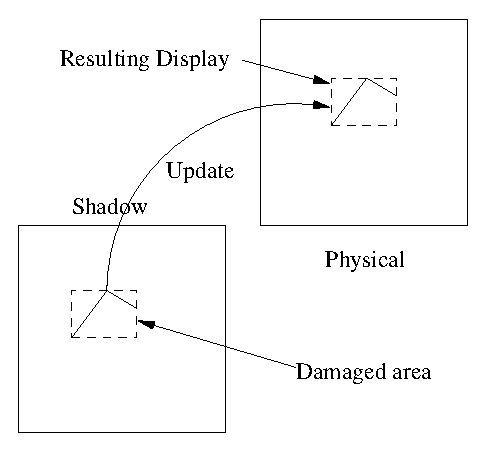
\epsfig{figure=shadow.eps}
\caption{Shadow Frame Buffer Operation}
\label{shadow.figure}
\end{center}
\end{figure}

The shadow frame buffer replaces the need for a complete rendering
implementation with a simple copy operation from the virtual frame buffer to
the hardware.  While rendering within the the shadow frame buffer cannot be
accelerated with the video hardware, the fact that the frame buffer lives in
regular memory and not across a PCI or AGP bus means that performance is
generally acceptable.  Because damaged regions are batched together during
periodic updates, the bandwidth of the bus doesn't significantly impact
overall performance.

RandR takes this shadow frame buffer implementation and creates a
virtual frame buffer for each depth not supported by the hardware.  As
seen in Figure~\ref{multi.figure}, copying the data from the virtual
frame buffer to the hardware involves converting the format of the
data to match the hardware, but as the original pixel data are
preserved in the shadow frame buffer, the display remains correct even
in the presence of complicated raster operations.  Depths supported by
the hardware remain implemented directly on the hardware with no
intermediate shadow frame buffer.  While this architecture could use
the additional frame buffers to eliminate some window damage, the
current implementation doesn't perform this optimization.
\begin{figure}
\begin{center}
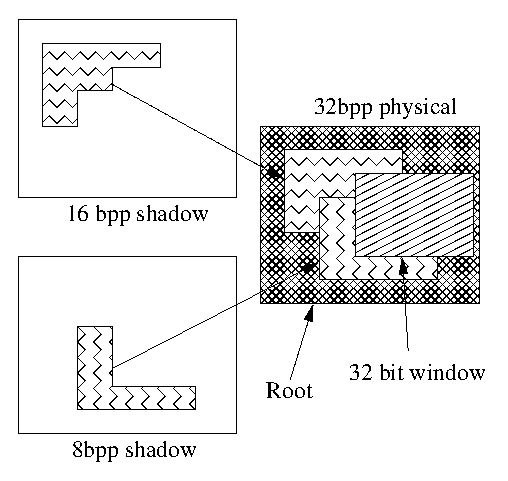
\epsfig{figure=multi.eps}
\caption{Supporting Multiple Depths}
\label{multi.figure}
\end{center}
\end{figure}

Using the shadow frame buffer in this way presumes that the X server can
already render to the necessary formats.  One recent addition to the XFree86
X server is ``fb'', a new implementation of simple frame buffer rendering
code.  By taking advantage of changes in the relationship between CPU and
memory performance, fb packs support for all X pixel sizes into a single
implementation.  This permits every X server to support all pixel sizes
without any effort, something which had been quite difficult in the past.
RandR takes advantage of this to provide simultaneous support for all of the
displayable pixel sizes.

Displaying the contents of these shadow frame buffers involves
converting the pixel values from one format to another format while
preserving the RGB values.  The Render extension already provides this
capability; all operations within that extension accept operands in arbitrary
formats.  RandR takes advantage of this functionality to perform the format
conversion when updating the hardware frame buffer with the contents of the
virtual frame buffers in.

\subsection{Rotating the Screen}

As hardware doesn't generally support changing the order that pixels are
read out of memory when generating the screen image, rotating the screen
involves changing the software to rotate the image within the frame buffer.

There are two possible implementations for this; the most obvious is to
rotate all of the rendering requests directed at the screen.  This turns out
to be somewhat complicated as there are many operations that involve
interactions between the screen and off-screen data and each one must rotate
the data.

While this may eventually be implemented, the current RandR implementation
uses the shadow frame buffer code as described above to keep a copy of the
screen in ``normal'' format; updates to the hardware frame buffer rotate the
image to orient the view correctly.  This implementation causes a slight
loss of performance as no rendering is accelerated and also uses
additional main memory for a copy of the frame bufffer.

\subsection{Changing the Screen Size and Depth}

The initial implementation for RandR has been done using the Tiny-X
architecture within the XFree86 X server.  This alternate driver mechanism
provides a minimal X server which eases development of new extensions
involving interactions between the device drivers and the extension.  RandR
requires some significant interactions to switch screen sizes and depths.
The intent is to migrate this architecture into the core XFree86 X server
when the interfaces have stabilized.

Tiny-X already supports dynamically reconfiguring the size and depth of the
video hardware; this capability is exported to the user by exposing multiple
``screens'' sharing the same physical video card.  Activating a new screen
involves disabling rendering to the old screen, reprogramming the video
hardware and enabling rendering for windows on the new screen.

Extending this to support RandR is straightforward: disable rendering to
the current screen, reprogram the hardware for the new configuration and
re-enable rendering.  When the depth changes, virtual frame buffers for the
old hardware depth become the targets for rendering at those depths. 
The new depth receives direct access to the hardware while it's virtual
frame buffer is disposed of.

\subsection{X Library Implementation}

We envision Xlib will always select for RRScreenChange events on all
screens, and that it will change the screen structure automatically
when such events arrive. (We will experimentally determine if this
seems to confuse clients.  By making the restriction that the default
depth and visual cannot change when a screen is changed, we believe
most clients will not need modification to support screen changes.)

We expect that most clients and toolkits will be oblivious to changes
to the screen stucture, as they generally use the values in the
connections Display structure directly.  By updating on the fly, we
believe pop-up menus and other pop up windows will position themselves
correctly in the face of screen configuration changes (the issue is
ensuring that pop-ups are visible on the reconfigured screen).

Advanced toolkits may wish to use the facilities of the extension
to determine which visuals are accelerated, and possibly change to
use them.

\section{The RandR Extension}

The extension itself is short enough that the inclusion of most of it
is worthwhile (we have elided the encoding). The version in this paper
is Version .97, and is not (yet) a standard of any kind, and is
certain to change before being finalized.  We expect it is likely some
additional change may be required as we gain implementation experience.

The specification methodology follows that of other X Window System
protocol design specifications.

The visuals advertised by an X server can never change.  This is to
prevent confusion of naive applications that may presume that the visual
type and depth of the root is fixed for all time: instead, the X server will
rerender the windows on a changed depth, though performance may be degraded
unless the client afterwards selects a visual belived to be hardware
accelerated (by being in the group of visuals resident in the
frame buffer).

Note that much of this design is provided to enable hot-swapping of
display cards, which can already occur on handheld computers using PCMCIA
and may occur in the future on other busses. Our experience over X's history
is that items we thought were static have often become dynamic as technology
changes, so we designed RandR with the presumption that almost anything about
the X server could change.

\subsection{Types}

The following types are used in the request and event definitions in
subsequent sections:

\begin{Xtype}
\Xenum{ROTATION} \{ 0, 90, 180, 270 \}. Degrees clockwise rotation
from native frame buffer orientation
\Xdecl{VISUALGROUP} LISTofVISUALID
\Xdecl{VISUALGROUPID} CARD16 index into VISUALGROUP
\Xdecl{GROUPofVISUALGROUP} LISTofVISUALGROUPID
\Xdecl{GROUPofVISUALGROUPID} CARD16 index into GROUPofVISUALGROUP
\Xstruct{SIZE} [width-in-pixels: CARD16\par
height-in-pixels: CARD16\par
width-in-mm: CARD16\par
height-in-mm: CARD16\par
visual-group-id: GROUPofVISUALGROUPID]
\Xdecl{SIZEID} CARD16 index into LISTofSIZE
\end{Xtype}

\subsection{Requests}

\begin{Xrequest}{RRQueryVersion}
\Xparam{clientMajorVersion} CARD16
\Xparam{clientMinorVersion} CARD16
\Xreply
\Xparam{serverMajorVersion} CARD16
\Xparam{serverMinorVersion} CARD16
\end{Xrequest}

The version numbers are an escape hatch in case future revisions of
the protocol are necessary.  The major version must increment for
incompatible changes, and the minor version SHOULD increment for small
upward compatible changes. Unrecognized requests or extra arguments to
a request within a major version MUST be ignored.  Barring changes,
the major version will be 1, and the minor version will be 0.

A server may support multiple versions of the extension: the reported
version is the one which will be used.

\begin{Xrequest}{RRGetScreenInfo}
\Xparam{window} Window
\Xreply
\Xparam{root} Window
\Xparam{visual-group} LISTofVISUALGROUP
\Xparam{groups-of-visual-groups} LISTofGROUPofVISUALGROUP
\Xparam{sizes} LISTofSIZE
\Xparam{rotations} SETofROTATIONS
\Xparam{size-index} SIZEID
\Xparam{visual-group-index} VISUALGROUPID
\Xparam{rotation} ROTATION
\Xparam{timestamp} TIMESTAMP
\Xparam{config-timestamp} TIMESTAMP
\Xerror{Drawable}
\end{Xrequest}

This request returns possible configurations on the screen associated
with the specified drawable along with the current configuration.

The reply contains the root window of the screen indicated in the
drawable argument of the request.

Visual-group is the list of possible combinations of visuals that can
be resident in the frame buffer directly together.  For each of these
visual groups, when it is selected in RRSetScreenConfig, applications
can expect that any window using one of the visuals in that group will
be resident in the frame buffer. When resident in
the frame buffer, colors on the screen will accurately reflect the
expected colors.  Rendering to such visuals may be accelerated in
hardware and may provide more timely feedback for graphics requests.

Groups-of-visual-groups group visual groups together to describe the
various ways a frame buffer can hold pixel values.  For example,
common frame buffers can support windows of only one depth at a time.
Groups-of-visual-groups would then contain a visual group with all of
the 8-bit visuals, a visual group with all of the 16-bit visuals and a
visual group with all of the 24-bit visuals, while high end hardware
might be able to handle these simultaneously, in which there would
be a single group.

Sizes is the list of possible frame buffer sizes, each provide both
the linear physical size of the screen and the pixel size.  Each size
also contains an index into the groups-of-visual-groups parameter.
This allows different sizes to support different possible frame buffer
configurations.  For example, a frame buffer with limited memory might
support 32-bit windows only at sizes less than 1152x900 pixels; sizes
greater than that would use a group-of-visual-groups not containing
the 32-bit visuals.

Rotations lists the supported orientations of the frame buffer relative to
the natural screen orientation.

Modern toolkits SHOULD use RRScreenChangeSelectInput to be notified
via a RRScreenChangeNotify event, so that they can change visual types
and/or depths and likely continue to receive the benefits of hardware
acceleration.

Size-index, visual-group-index and rotation indicate the size,
visual-group and rotation currently in use.

The config-timestamp indicates when the screen configuration
information last changed: requests to set the screen will fail unless
the timestamp indicates that the information the client is using is up
to date, to ensure clients can be well behaved in the face of race
conditions. Similarly, timestamp indicates when the configuration was
last set, and must both must be up to date in a call to
RRSetScreenConfig for it to succeed.

\begin{Xrequest}{RRSetScreenConfig}
\Xparam{draw} DRAWABLE
\Xparam{size-index} SIZEID
\Xparam{visual-group-index} VISUALGROUPID
\Xparam{rotation} ROTATION
\Xparam{timestamp} TIMESTAMP
\Xparam{config-timestamp} TIMESTAMP
\Xreply
\Xparam{new-timestamp} TIMESTAMP
\Xparam{config-timestamp} TIMESTAMP
\Xparam{success} BOOL
\Xparam{root} WINDOW
\Xerror{Value, Drawable}
\end{Xrequest}

If the timestamp in this request is less than the time when the
configuration was last successfully set, the request is ignored and
False returned in success.  If the config-timestamp in this request is
not equal to when the server's screen configurations last changed, the
request is ignored and False returned in success.  This could occur if
the screen changed since you last made a RRGetScreenInfo request,
perhaps by a different piece of display hardware being installed..
Rather than allowing an incorrect call to be executed based on stale
data, the server will ignore the request.

If the request succeeds, this request sets the screen to the specified
size and sets the active visual group to that specified by
visual-group-index, and the rotation to the specified rotation. If the
requests succeeds, the new-time-stamp is returned containing the time
when the screen configuration was changed and config-timestamp is
returned to indicate when the possible screen configurations were last
changed, and success is set to True.  The root window for the screen
indicated by the drawable argument is also returned.

BadValue errors are generated if the rotation is not an allowed
rotation. BadValue errors are generated, if, when the timestamps would
allow the operation to succeed, the visual-group-index or size-index
are not possible (out of range).

\begin{Xrequest}{RRScreenChangeSelectInput}
\Xparam{window} WINDOW
\Xparam{enable} BOOL
\Xerror{Value, Window}
\end{Xrequest}

Requests that RRScreenChange events of screen changes of the screen
associated with the drawable be delivered to the specified window. (whew!)

Clients may then choose to create new resources or use other visuals
that have hardware acceleration available that take advantage of
the new screen configuration.

\subsection{Events}

To reconfigure the root window, use the RRSetScreen request defined
above.

\begin{Xrequest}{RRScreenChangeNotify}
\Xparam{root} WINDOW
\Xparam{window} WINDOW
\Xparam{size-index} SIZEID
\Xparam{visual-group-index} VISUALGROUPID
\Xparam{rotation} ROTATION
\Xparam{config-timestamp} TIMESTAMP
\Xparam{timestamp} TIMESTAMP
\Xparam{new-width-in-pixels, new-height-in-pixels} CARD16
\Xparam{new-width-in-mm, new-height-in-mm} CARD16
\end{Xrequest}

This event is delivered to clients selecting for notification with
RRScreenChangeSelectInput requests.

This event is delivered clients selecting for notification with
RRScreenChangeSelectInput.   Size-index indicates which size is active.
Visual-group-index indicates the current visual group.  The returned
window is the window requsting notification.

This event is sent whenever the screen's visual group is changed, or
if a new screen configuration becomes available that was not available
in the past.  In this case (config-timestamp in the event not being
equal to the config-timestamp returned in the last call to
RRGetScreenInfo), the client MUST call RRGetScreenInfo to update its
view of possible screen configurations to have a correct view of
possible screen organizations. Timestamp is set to when the active
screen configuration was changed.

This call also returns the size in pixels and millimeters of the
screen and the root window of the screen which has changed.

\section{History and Status}

This extension has been designed and significant external review input
incorporated. A prototype implementation is functioning in the TinyX X
implementation.\cite{tinyx}


\section{Future Work}

The XAA~\cite{xaa} implementation of the full XFree86 will need
extension to fully support this protocol extension, prototyped in the
TinyX framework.

Toolkits will need updating to support RandR to take advantage of
accelerated visual type information to ensure highest possible
performance.

Window managers will need to support this extension to layout the
screen in some fashion when the size changes to ensure applications
are appropriately visible.

There are very entertaining user interface possibilities for moving
applications between screens, particularly once systems become aware
of resources available in their nearby environment. A free, off the
wall (or maybe on the wall), idea might be given a handheld computer
with accelerometers such as Itsy\cite{Itsy} you might almost literally
throw windows from one screen to another.  Other hacks are left to the
bizarre nature of your own imagination.

\section*{Acknowledgments}

The authors would like to thank their respective employers, Compaq and SuSE,
for support of open source software development and the XFree86 project for
it's continuing advancement of the X Window System.  Additional thanks go to
Carl Worth and Alexander Guy for their help in editing the manuscript.

\bibliographystyle{alpha}
\bibliography{./randr}
\end{document}
